% Notes Template
% Template version used: v0.3
% https://github.com/rnsavinelli/notes-template
%
%!TEX encoding = UTF-8 Unicode

% Document-class options:
\documentclass[letter]{article}

% Package includes and formatting settings -----------
% ----------------------------------------------------

% LaTeX Font encoding - 8-bit fonts
\usepackage[T1]{fontenc}
\usepackage[utf8]{inputenc}
\usepackage[sc, osf]{mathpazo}

\usepackage{hyperref}

% These settings should be modified / deleted /
\def\authorsname{Mr./Mrs. Author}
\def\authorswebsite{}
\def\course{\LaTeX}
\def\courseyear{}
\def\typeoffile{Template}
\def\university{}

% PDF Settings
\hypersetup{
    pdfauthor = {\authorsname},
    pdfkeywords = {-},
    pdftitle = {\course \ \typeoffile},
    pdfsubject = {-},
    pdfcreator={TeX}
}

% HREF settings
\hypersetup{
    colorlinks = true,
    urlcolor = blue,
    linkcolor = black
}

% LaTeX' own graphics handling
\usepackage{graphicx}
\graphicspath{ {./images/} }

% AMS-LaTeX extensions for mathematical typesetting.
\usepackage{amsmath,amsthm,amsfonts,amssymb,mathrsfs}

% Document format and settings -----------------------
% ----------------------------------------------------
\usepackage[left=.75in, right=.75in, bottom=1in, top=1in]{geometry}

% Better spacing between lines
\usepackage{parskip}

\setlength\parindent{0em}
%\pagenumbering{roman}

\usepackage{chngcntr}
\counterwithin*{equation}{section}

% Title, section, and topic formatting
\usepackage{titlesec}

\titleformat{\section}{\bfseries\Large}{}{0em}{}
\titleformat{\subsection}{\bfseries\large}{}{0em}{}
\titleformat{\subsubsection}{\bfseries\normalsize}{}{0em}{}

% \today commands
\usepackage{datetime}

\usepackage{lipsum}

% Content of the document ----------------------------
% ----------------------------------------------------

\begin{document}

\title{\bfseries \course \ \typeoffile}
\author{\authorsname}
\date{}

\maketitle

% Include as many files as needed. This approach is taken to reduce the amount of
% information contained in this very same document. It is not mandatory to use external
% files to add your content but it is highly recommended.
%
% \input is preferred over \include since the latter automatically appends a page break.

%!TEX root = notex.tex

\section{Some Information}

\lipsum[0-1]

\begin{equation}
    \vec{E} = - \left( \frac{\partial V}{\partial x} \ \hat{x} + \frac{\partial V}{\partial y} \ \hat{y} + 
    \frac{\partial V}{\partial z} \ \hat{z} \right) = - (\vec{E_{x}} + \vec{E_{y}} + \vec{E_{z}})
\end{equation}

\lipsum[2-3]

\subsection{A subsection}

\lipsum[4-5]

\begin{figure}[h]
    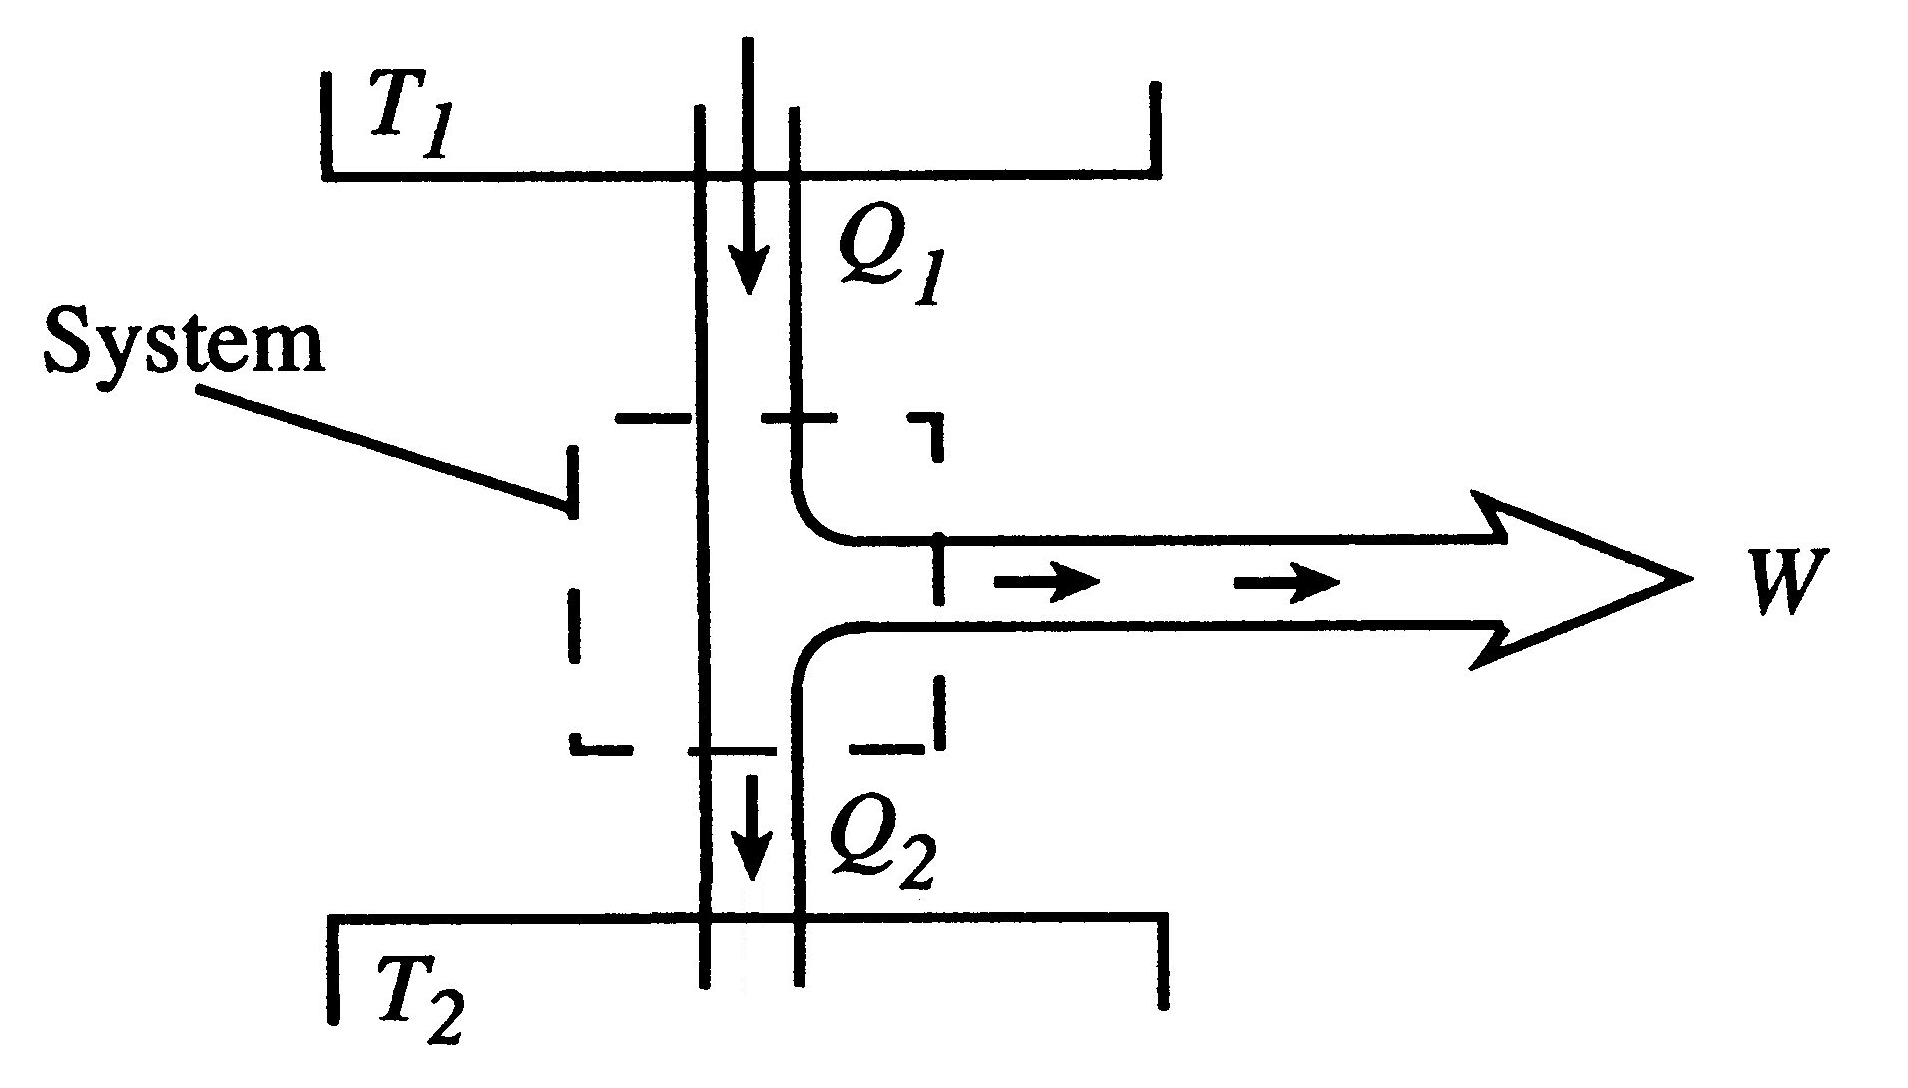
\includegraphics[width=0.4\textwidth]{second_law.png}
    \centering
    \caption{Lorem ipsum}
    \label{fig:lorem-ipsum}
\end{figure}

\lipsum[6]

\subsection{Another subsection}

\lipsum[7]

\begin{align*}
    \Delta U = W_{Point} = \int_{r_{a}}^{r_{b}} \vec{F_{Point}} \ \vec{dr}
\end{align*}    

\begin{equation}
    \Delta U = W_{Point} = - \int_{r_{a}}^{r_{b}} \vec{F_{Elec}} \ \vec{dr}
\end{equation} 

\lipsum[8]

\section{More information}

\lipsum[9-11]

\subsection{And another subsection}

\lipsum[11-13]


% Closing of the document ----------------------------
% ----------------------------------------------------
%\newpage

%\section{About This Document}

%Maybe add some bibliography or additional information.

%Last updated: {\today}.

\end{document}

% End of the document --------------------------------
% ----------------------------------------------------
